Przed przystąpieniem do wykonania projektu, wskazane jest opisanie założeń projektowych i krótki spis narzędzi wykorzystanych do ich zrealizowania. Założenia podzielone zostały na kilka podsekcji, po jednej dla każdej części projektu. Wyjaśnienie poszczególnych części/modułów znajduje się w Rozdziale \ref{ch:project}. 

\section{Założenia}
\label{ch:zalozenia}

\subsection*{Dla układu elektronicznego}
\begin{itemize}
    \item 2 silniki DC (ang.~\english{Direct Current})
    \item sterownik silników
    \item czujnik laserowy z przodu pojazdu
    \item enkodery magnetyczne do pomiaru położenia wałów silników
    \item sterowanie przy użyciu mikroprocesora
    \item LED (ang.~\english{Light Emitting Diode}) sygnalizujący stan oprogramowania mikroprocesora
    \item głośnik sygnalizujący stan oprogramowania mikroprocesora
    \item bezpieczniki zabezpieczające układ elektroniczny
    \item przełączniki źródeł prądowych
\end{itemize}

\subsection*{Dla modelu pojazdu}
\begin{itemize}
    \item możliwa jazda do przodu, tyłu oraz skręcanie jak w samochodzie osobowym
    \item 4 koła, kilka zestawów rozmiarów dla różnorodności eksperymentalnej
    \item modułowość pozwalająca na modyfikację w razie potrzeby
    \item projekt wizualny podobny do samochodu osobowego
    \item obudowa wydrukowana na drukarce 3D
\end{itemize}

\subsection*{Dla oprogramowania mikroprocesora}
\begin{itemize}
    \item system FreeRTOS (ang.~\english{Real Time Operating System})
    \item wykonanie w języku C++
    \item klient i serwer UDP (ang.~\english{User Datagram Protocol})
    \item interpretacja danych z~ramek pakietów UDP
    \item sterowanie możliwe w~układzie otwartym lub zamkniętym
    \item wartość zadana odbierana z aplikacji mobilnej przez Wi-Fi (ang.~\english{Wireless Fidelity})
    \item rozpoczęcie i zakończenie pomiaru na komendę z aplikacji mobilnej
    \item awaryjne zakończenie pomiaru w przypadku rozłączenia Wi-Fi
    \item odczytywanie kierunku i położenia enkoderów
    \item synchronizacja silników
    \item obliczanie sygnałów sterujących silników regulatorami PID
    \item plik konfiguracyjny
\end{itemize}

\subsection*{Dla aplikacji mobilnej}
\begin{itemize}
    \item działanie na systemie Android
    \item prostota wykonania i użytkowania
    \item krótki czas tworzenia (ang.~\english{development})
    \item klient i serwerUDP
    \item interpretacja danych z ramek pakietów UDP
    \item zmienny docelowy adres IP (ang.~\english{Internet Protocol}) 
    \item parametryzacja regulatorów PID
    \item ustawianie wartości zadanej i prędkości
\end{itemize}

\subsection*{Dla skryptu odbierającego dane}
\begin{itemize}
    \item działanie na systemie Windows
    \item wykonanie w~języku Python
    \item serwer UDP
    \item interpretacja danych z~ramek pakietów UDP
    \item zapis danych do pliku .csv (ang.~\english{Comma-Separated Values})
    \item działanie w~pętli; możliwość odbioru wielu pomiarów
\end{itemize}

\subsection*{Dla skryptu wizualizujacego dane}
\begin{itemize}
    \item działanie na systemie windows
    \item odczytywanie danych z~pliku .csv
    \item wizualizacja odczytanych danych (tworzenie wykresów)
    \item zapisywanie wykresów do pliku .eps (ang.~\english{Encapsulated PostScript})
\end{itemize}

\newpage

\section{Narzędzia}
\label{ch:narzedzia}
% ============ hardware ============ %
\subsection*{Narzędzia fizyczne}

\begin{itemize}
    \item Zestaw lutowniczy 
    Lutowanie to proces łączenia elementów elektronicznych przez stopienie spoiwa lutowniczego na przylegających do siebie elementach metalowych, a~następnie jego zastygnięcie. Do lutowania wykorzystane zostały następujące narzędzia:

    \begin{itemize}
        \item lutownica transformatorowa 100~W typu B % kim był Transformatorov?
        \item topnik w~żelu
        \item plecionka do rozlutowywania
        \item cyna lutownicza bezołowiowa z~3.8\% srebra
        \item alkohol izopropylowy 100\%
        \item zestaw przewodów typu prototypowego (ang.~\english{jumper wires})
        \item folia aluminiowa
    \end{itemize}

    Lutownica jest, oprócz drukarki 3D, najważniejszym narzędziem użytym w~projekcie.

    \item Czarna taśma izolacyjna o wielofunkcyjnym zastosowaniu --- izolacja elementów elektrycznych, ale również czynnik pomocniczy, zwiększający tarcie i~łączący luźne elementy.

    \item Pistolet do kleju na gorąco posłużył do przytwierdzania elementów w~miejscu.

    \item Multimetr do pomiaru wielkości elektrycznych. W~projekcie użyto modelu UNI-T M830BUZ z~funkcją mierzenia napięcia, natężenia, rezystancji i~ciągłości.

    \item Drukarka 3D (Rysunek~\ref{fig:drukarka}), na której wydrukowano obudowę oraz koła pojazdu.
    \begin{center}
        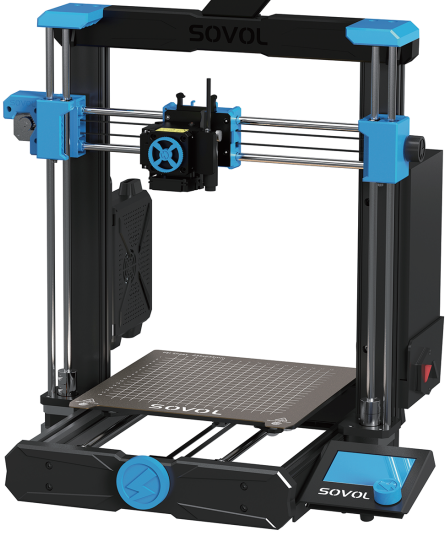
\includegraphics[scale=0.5]{images/printer.png}
        \captionof{figure}{Drukarka 3D model Sovol SV06 (Bibliografia:~\cite{bib:printer})}
        \label{fig:drukarka}
    \end{center}
\end{itemize}

% ============ software ============ %
\subsection*{Oprogramowanie}

\subsubsection*{Visual Studio Code}
Do napisania oprogramowania mikroprocesora oraz pracy inżynierskiej użyta została platforma Visual Studio Code, z~rozszerzeniami LaTeX Workshop i~PlatformIO IDE.

\subsubsection*{MATLAB}
MATLABa użyto w~celu wizualizacji danych otrzymanych z~pojazdu.

\subsubsection*{GitHub}
GitHub posłużył jako system kontroli wersji, zarówno do kodu mikroprocesora, jak i~do skryptów pomocniczych i~pracy inżynierskiej.

\subsubsection*{MIT App Inventor}
MIT App Inventor wykorzystany został do stworzenia aplikacji na system Android.

\subsubsection*{Autodesk Inventor}
W Inventorze zaprojektowano modele 3D pojazdu do druku 3D.

\subsection*{Paint.NET}
Program do obróbki graficznej, utworzono w nim schemat układu elektronicznego.